%!TEX root = Main.tex
\documentclass[Main]{subfiles}

\begin{document}

\subsection{Class diagrams}

The class diagram for the client is shown on figure \ref{fig:clientuml}. The only classes developed for the client is for the event handlers:  \code{PatientValSender\_EventHandler}, \code{LogSender\_EventHandler}, \code{AlarmSender\_EventHandler}.

\begin{figure}[hbtp]
\centering
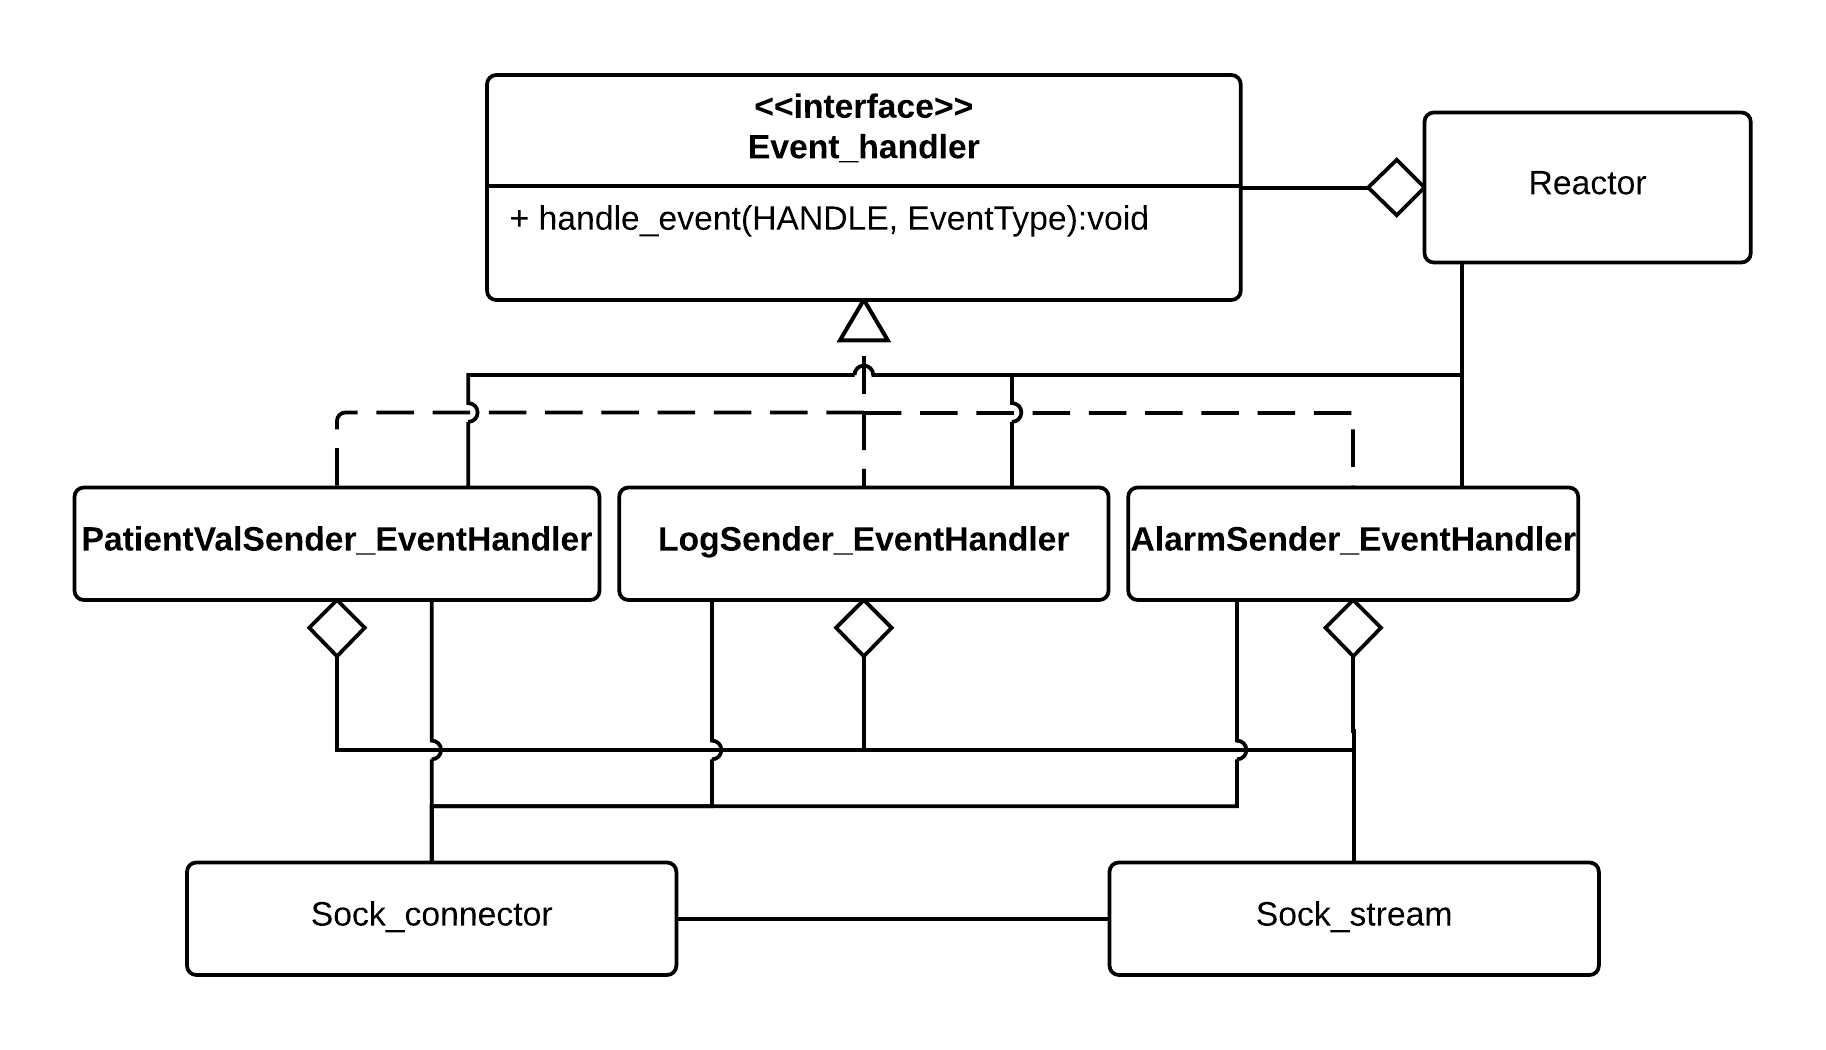
\includegraphics[width=1.0\textwidth]{Assignment1clientclassdiag}
\caption{Class diagram for client.}
\label{fig:clientuml}
\end{figure}

\end{document}